\documentclass{beamer}

\DeclareOptionBeamer{slidesperpage}{2}

%\usefonttheme[onlymath]{serif}
\mode<presentation>
{
  \usetheme{default}
  % or ...

  \setbeamersize{text margin left=1em,text margin right=1em}
  \setbeamercovered{invisible}
  \setbeamertemplate{footline}
  {
  \begin{beamercolorbox}[wd=\paperwidth,ht=2.5ex,dp=1ex,left]{date in head/foot}%
    \usebeamerfont{date in head/foot}
    \hspace*{2ex}CS 422
    \hspace{\stretch{100}}
    Hal Daum\'e III (UMD)
    \hspace{\stretch{100}}
    \makebox[0in][b]{\insertframenumber{} / \inserttotalframenumber}\hspace*{2ex}
  \end{beamercolorbox}
%  \begin{beamercolorbox}[wd=\paperwidth,ht=2.25ex,dp=1ex,right]{date in head/foot}%
%    \usebeamerfont{date in head/foot}
%    \insertframenumber{} / \inserttotalframenumber\hspace*{2ex} 
%  \end{beamercolorbox}
  }
  % or whatever (possibly just delete it)
}


\usepackage[english]{babel}
% or whatever

\usepackage[latin1]{inputenc}
% or whatever

\usepackage{graphicx}
\usepackage{times}
\usepackage{xcolor}
\usepackage[T1]{fontenc}

\usepackage{natbib}
\usepackage{haldefs}
\usepackage{notes-slides}
\bibliographystyle{plainnat}
\bibpunct{[}{]}{,}{a}{,}{,}

% Or whatever. Note that the encoding and the font should match. If T1
% does not look nice, try deleting the line with the fontenc.

\definecolor{DarkGreen}   {rgb}{0,0.5,0}
\definecolor{DarkBlue}    {rgb}{0,0.0,0.5}
\definecolor{LightGray}   {rgb}{0.8,0.8,0.8}


\newcommand{\vsp}{\vspace{1em}}
\newcommand{\hsp}{\hspace{1em}}
\newcommand{\blue}[1]{{\color{blue}#1}}
\newcommand{\green}[1]{{\color{DarkGreen}#1}}
\newcommand{\black}[1]{{\color{black}#1}}
\newcommand{\red}[1]{{\color{red}#1}}

\usecolortheme{default}   % default, albatross, crane, dove, fly, seagull
\setbeamercolor{frametitle}{fg=DarkBlue,bg=LightGray}
\beamertemplatenavigationsymbolsempty

\begin{document}

\begin{frame}
\only<1>{\green{\LARGE\bf Pixel Color Values}}
\only<2-6>{\green{\LARGE\bf Image Textures}}
\only<7-11>{\green{\LARGE\bf Image Shape}}
\only<12-16>{\green{\LARGE\bf Actual Images}}

\vsp
\begin{tabular}{|c|c|c|}
\hline
Object 1: & Object 2: & Object 3: \\
\only<1-1>{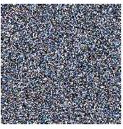
\includegraphics[height=.35\textheight]{object1-color.png}}
\only<2-6>{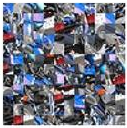
\includegraphics[height=.35\textheight]{object1-texture.png}}
\only<7-11>{
\includegraphics[height=.30\textheight]{object1-shape.png}}
\only<12-16>{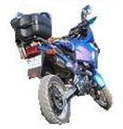
\includegraphics[height=.30\textheight]{object1-image.png}}
 &
\only<1-2>{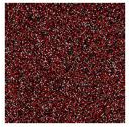
\includegraphics[height=.35\textheight]{object2-color.png}}
\only<3-7>{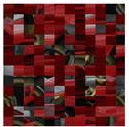
\includegraphics[height=.35\textheight]{object2-texture.png}}
\only<8-12>{
\includegraphics[height=.15\textheight]{object2-shape.png}}
\only<13-16>{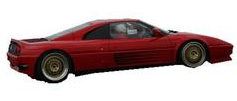
\includegraphics[height=.15\textheight]{object2-image.png}}
 &
\only<1-3>{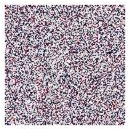
\includegraphics[height=.35\textheight]{object3-color.png}}
\only<4-8>{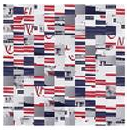
\includegraphics[height=.35\textheight]{object3-texture.png}}
\only<9-13>{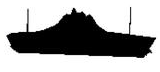
\includegraphics[height=.15\textheight]{object3-shape.png}}
\only<14-16>{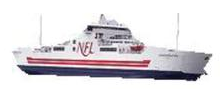
\includegraphics[height=.15\textheight]{object3-image.png}}
 \\
\hline
Object 4: & Object 5: & \\
\only<1-4>{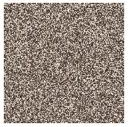
\includegraphics[height=.35\textheight]{object4-color.png}}
\only<5-9>{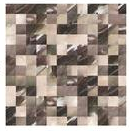
\includegraphics[height=.35\textheight]{object4-texture.png}}
\only<10-14>{
\includegraphics[height=.30\textheight]{object4-shape.png}}
\only<15-16>{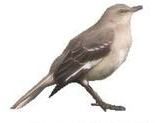
\includegraphics[height=.30\textheight]{object4-image.png}}
 &
\only<1-5>{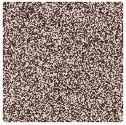
\includegraphics[height=.35\textheight]{object5-color.png}}
\only<6-10>{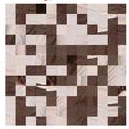
\includegraphics[height=.35\textheight]{object5-texture.png}}
\only<11-15>{
\includegraphics[height=.30\textheight]{object5-shape.png}}
\only<16>{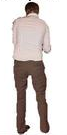
\includegraphics[height=.30\textheight]{object5-image.png}}
 &
 \\
\hline
\end{tabular}
\end{frame}

% \begin{frame}
% \frametitle{Feature set = texture distribution}

% \begin{tabular}{|c|c|c|}
% \hline
% Object 1: & Object 2: & Object 3: \\
% 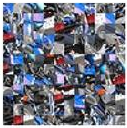
\includegraphics[height=.35\textheight]{object1-texture.png} &
% 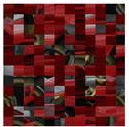
\includegraphics[height=.35\textheight]{object2-texture.png} &
% 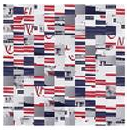
\includegraphics[height=.35\textheight]{object3-texture.png} \\
% \hline
% Object 4: & Object 5: & \\
% 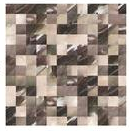
\includegraphics[height=.35\textheight]{object4-texture.png} &
% 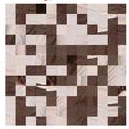
\includegraphics[height=.35\textheight]{object5-texture.png} & \\
% \hline
% \end{tabular}
% \end{frame}

% \begin{frame}
% \frametitle{Feature set = shape distribution}

% \begin{tabular}{|c|c|c|}
% \hline
% Object 1: & Object 2: & Object 3: \\
% 
\includegraphics[height=.35\textheight]{object1-shape.png} &
% 
\includegraphics[height=.15\textheight]{object2-shape.png} &
% 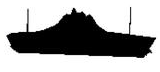
\includegraphics[height=.15\textheight]{object3-shape.png} \\
% \hline
% Object 4: & Object 5: & \\
% 
\includegraphics[height=.35\textheight]{object4-shape.png} &
% 
\includegraphics[height=.35\textheight]{object5-shape.png} & \\
% \hline
% \end{tabular}
% \end{frame}

% \begin{frame}
% \frametitle{Actual Image}

% \begin{tabular}{|c|c|c|}
% \hline
% Object 1: & Object 2: & Object 3: \\
% 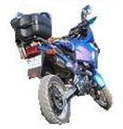
\includegraphics[height=.35\textheight]{object1-image.png} &
% 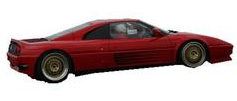
\includegraphics[height=.15\textheight]{object2-image.png} &
% 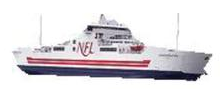
\includegraphics[height=.15\textheight]{object3-image.png} \\
% \hline
% Object 4: & Object 5: & \\
% 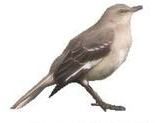
\includegraphics[height=.35\textheight]{object4-image.png} &
% 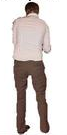
\includegraphics[height=.35\textheight]{object5-image.png} & \\
% \hline
% \end{tabular}
% \end{frame}


\end{document}
